\documentclass[hyperref={colorlinks=true}]{beamer}

\mode<presentation>
{
	\usetheme{Warsaw}
	\setbeamercovered{transparent}
}
\usepackage[english]{babel}
\usepackage[latin1]{inputenc}

\usepackage{longtable}

\usepackage{sphinx}

\makeatletter
\def\PYG@reset{\let\PYG@it=\relax \let\PYG@bf=\relax%
    \let\PYG@ul=\relax \let\PYG@tc=\relax%
    \let\PYG@bc=\relax \let\PYG@ff=\relax}
\def\PYG@tok#1{\csname PYG@tok@#1\endcsname}
\def\PYG@toks#1+{\ifx\relax#1\empty\else%
    \PYG@tok{#1}\expandafter\PYG@toks\fi}
\def\PYG@do#1{\PYG@bc{\PYG@tc{\PYG@ul{%
    \PYG@it{\PYG@bf{\PYG@ff{#1}}}}}}}
\def\PYG#1#2{\PYG@reset\PYG@toks#1+\relax+\PYG@do{#2}}

\def\PYG@tok@gu{\let\PYG@bf=\textbf\def\PYG@tc##1{\textcolor[rgb]{0.50,0.00,0.50}{##1}}}
\def\PYG@tok@gt{\def\PYG@tc##1{\textcolor[rgb]{0.00,0.25,0.82}{##1}}}
\def\PYG@tok@gs{\let\PYG@bf=\textbf}
\def\PYG@tok@gr{\def\PYG@tc##1{\textcolor[rgb]{1.00,0.00,0.00}{##1}}}
\def\PYG@tok@cm{\let\PYG@it=\textit\def\PYG@tc##1{\textcolor[rgb]{0.25,0.50,0.56}{##1}}}
\def\PYG@tok@vg{\def\PYG@tc##1{\textcolor[rgb]{0.73,0.38,0.84}{##1}}}
\def\PYG@tok@m{\def\PYG@tc##1{\textcolor[rgb]{0.13,0.50,0.31}{##1}}}
\def\PYG@tok@mh{\def\PYG@tc##1{\textcolor[rgb]{0.13,0.50,0.31}{##1}}}
\def\PYG@tok@go{\def\PYG@tc##1{\textcolor[rgb]{0.19,0.19,0.19}{##1}}}
\def\PYG@tok@ge{\let\PYG@it=\textit}
\def\PYG@tok@gd{\def\PYG@tc##1{\textcolor[rgb]{0.63,0.00,0.00}{##1}}}
\def\PYG@tok@il{\def\PYG@tc##1{\textcolor[rgb]{0.13,0.50,0.31}{##1}}}
\def\PYG@tok@cs{\def\PYG@tc##1{\textcolor[rgb]{0.25,0.50,0.56}{##1}}\def\PYG@bc##1{\colorbox[rgb]{1.00,0.94,0.94}{##1}}}
\def\PYG@tok@cp{\def\PYG@tc##1{\textcolor[rgb]{0.00,0.44,0.13}{##1}}}
\def\PYG@tok@gi{\def\PYG@tc##1{\textcolor[rgb]{0.00,0.63,0.00}{##1}}}
\def\PYG@tok@gh{\let\PYG@bf=\textbf\def\PYG@tc##1{\textcolor[rgb]{0.00,0.00,0.50}{##1}}}
\def\PYG@tok@ni{\let\PYG@bf=\textbf\def\PYG@tc##1{\textcolor[rgb]{0.84,0.33,0.22}{##1}}}
\def\PYG@tok@nl{\let\PYG@bf=\textbf\def\PYG@tc##1{\textcolor[rgb]{0.00,0.13,0.44}{##1}}}
\def\PYG@tok@nn{\let\PYG@bf=\textbf\def\PYG@tc##1{\textcolor[rgb]{0.05,0.52,0.71}{##1}}}
\def\PYG@tok@no{\def\PYG@tc##1{\textcolor[rgb]{0.38,0.68,0.84}{##1}}}
\def\PYG@tok@na{\def\PYG@tc##1{\textcolor[rgb]{0.25,0.44,0.63}{##1}}}
\def\PYG@tok@nb{\def\PYG@tc##1{\textcolor[rgb]{0.00,0.44,0.13}{##1}}}
\def\PYG@tok@nc{\let\PYG@bf=\textbf\def\PYG@tc##1{\textcolor[rgb]{0.05,0.52,0.71}{##1}}}
\def\PYG@tok@nd{\let\PYG@bf=\textbf\def\PYG@tc##1{\textcolor[rgb]{0.33,0.33,0.33}{##1}}}
\def\PYG@tok@ne{\def\PYG@tc##1{\textcolor[rgb]{0.00,0.44,0.13}{##1}}}
\def\PYG@tok@nf{\def\PYG@tc##1{\textcolor[rgb]{0.02,0.16,0.49}{##1}}}
\def\PYG@tok@si{\let\PYG@it=\textit\def\PYG@tc##1{\textcolor[rgb]{0.44,0.63,0.82}{##1}}}
\def\PYG@tok@s2{\def\PYG@tc##1{\textcolor[rgb]{0.25,0.44,0.63}{##1}}}
\def\PYG@tok@vi{\def\PYG@tc##1{\textcolor[rgb]{0.73,0.38,0.84}{##1}}}
\def\PYG@tok@nt{\let\PYG@bf=\textbf\def\PYG@tc##1{\textcolor[rgb]{0.02,0.16,0.45}{##1}}}
\def\PYG@tok@nv{\def\PYG@tc##1{\textcolor[rgb]{0.73,0.38,0.84}{##1}}}
\def\PYG@tok@s1{\def\PYG@tc##1{\textcolor[rgb]{0.25,0.44,0.63}{##1}}}
\def\PYG@tok@vc{\def\PYG@tc##1{\textcolor[rgb]{0.73,0.38,0.84}{##1}}}
\def\PYG@tok@sh{\def\PYG@tc##1{\textcolor[rgb]{0.25,0.44,0.63}{##1}}}
\def\PYG@tok@ow{\let\PYG@bf=\textbf\def\PYG@tc##1{\textcolor[rgb]{0.00,0.44,0.13}{##1}}}
\def\PYG@tok@mf{\def\PYG@tc##1{\textcolor[rgb]{0.13,0.50,0.31}{##1}}}
\def\PYG@tok@bp{\def\PYG@tc##1{\textcolor[rgb]{0.00,0.44,0.13}{##1}}}
\def\PYG@tok@c1{\let\PYG@it=\textit\def\PYG@tc##1{\textcolor[rgb]{0.25,0.50,0.56}{##1}}}
\def\PYG@tok@kc{\let\PYG@bf=\textbf\def\PYG@tc##1{\textcolor[rgb]{0.00,0.44,0.13}{##1}}}
\def\PYG@tok@c{\let\PYG@it=\textit\def\PYG@tc##1{\textcolor[rgb]{0.25,0.50,0.56}{##1}}}
\def\PYG@tok@sx{\def\PYG@tc##1{\textcolor[rgb]{0.78,0.36,0.04}{##1}}}
\def\PYG@tok@err{\def\PYG@bc##1{\fcolorbox[rgb]{1.00,0.00,0.00}{1,1,1}{##1}}}
\def\PYG@tok@kd{\let\PYG@bf=\textbf\def\PYG@tc##1{\textcolor[rgb]{0.00,0.44,0.13}{##1}}}
\def\PYG@tok@ss{\def\PYG@tc##1{\textcolor[rgb]{0.32,0.47,0.09}{##1}}}
\def\PYG@tok@sr{\def\PYG@tc##1{\textcolor[rgb]{0.14,0.33,0.53}{##1}}}
\def\PYG@tok@mo{\def\PYG@tc##1{\textcolor[rgb]{0.13,0.50,0.31}{##1}}}
\def\PYG@tok@kn{\let\PYG@bf=\textbf\def\PYG@tc##1{\textcolor[rgb]{0.00,0.44,0.13}{##1}}}
\def\PYG@tok@mi{\def\PYG@tc##1{\textcolor[rgb]{0.13,0.50,0.31}{##1}}}
\def\PYG@tok@gp{\let\PYG@bf=\textbf\def\PYG@tc##1{\textcolor[rgb]{0.78,0.36,0.04}{##1}}}
\def\PYG@tok@o{\def\PYG@tc##1{\textcolor[rgb]{0.40,0.40,0.40}{##1}}}
\def\PYG@tok@kr{\let\PYG@bf=\textbf\def\PYG@tc##1{\textcolor[rgb]{0.00,0.44,0.13}{##1}}}
\def\PYG@tok@s{\def\PYG@tc##1{\textcolor[rgb]{0.25,0.44,0.63}{##1}}}
\def\PYG@tok@kp{\def\PYG@tc##1{\textcolor[rgb]{0.00,0.44,0.13}{##1}}}
\def\PYG@tok@w{\def\PYG@tc##1{\textcolor[rgb]{0.73,0.73,0.73}{##1}}}
\def\PYG@tok@kt{\def\PYG@tc##1{\textcolor[rgb]{0.56,0.13,0.00}{##1}}}
\def\PYG@tok@sc{\def\PYG@tc##1{\textcolor[rgb]{0.25,0.44,0.63}{##1}}}
\def\PYG@tok@sb{\def\PYG@tc##1{\textcolor[rgb]{0.25,0.44,0.63}{##1}}}
\def\PYG@tok@k{\let\PYG@bf=\textbf\def\PYG@tc##1{\textcolor[rgb]{0.00,0.44,0.13}{##1}}}
\def\PYG@tok@se{\let\PYG@bf=\textbf\def\PYG@tc##1{\textcolor[rgb]{0.25,0.44,0.63}{##1}}}
\def\PYG@tok@sd{\let\PYG@it=\textit\def\PYG@tc##1{\textcolor[rgb]{0.25,0.44,0.63}{##1}}}

\def\PYGZbs{\char`\\}
\def\PYGZus{\char`\_}
\def\PYGZob{\char`\{}
\def\PYGZcb{\char`\}}
\def\PYGZca{\char`\^}
% for compatibility with earlier versions
\def\PYGZat{@}
\def\PYGZlb{[}
\def\PYGZrb{]}
\makeatother

% Ams stuff, nice equations and fonts ...
\usepackage{amsmath}
\usepackage{amsfonts}
\usepackage{amstext}
\usepackage{latexsym}
\usepackage{amssymb}
\usepackage{amsthm}
% yeah commutative diagrams
\usepackage{amscd}

% Basic graphics for including postscript files
\usepackage{graphics}
\usepackage{epsfig}

% Some more useful packages
\usepackage{verbatim}
% \usepackage{moreverb}


% Shows labels, useful during writing stage
%\usepackage{showkeys}


%\pagestyle{headings}

%------------------------------------

% other things i have found useful
\usepackage{url}
\usepackage{mathrsfs}

\usepackage{listings}

%---- homegrown latex macros ---------------
\renewcommand{\natural}{\mathbb{N}}
\newcommand{\real}{\mathbb{R}}
\newcommand{\complex}{\mathbb{C}}
\newcommand{\integer}{\mathbb{Z}}
\DeclareMathOperator{\D}{D}
\newcommand{\gradient}{\nabla}
\newcommand{\laplacian}{\Delta}
\newcommand{\boundary}{\partial}
\DeclareMathOperator{\diam}{diam}
\newcommand{\definedby}{\mathrel{\mathop:}=}
\DeclareMathOperator{\dist}{dist}
\DeclareMathOperator{\support}{supp}
\DeclareMathOperator{\image}{im}
\DeclareMathOperator{\trace}{tr}
\newcommand{\union}{\cup}
\newcommand{\intersection}{\cap}
\DeclareMathOperator{\diag}{diag}
\newcommand{\powerset}{\mathcal{P}}
\DeclareMathOperator{\argmin}{argmin}
\DeclareMathOperator{\graph}{graph}
\DeclareMathOperator{\linspan}{span}
\DeclareMathOperator{\esssup}{{ess sup}}
\DeclareMathOperator{\divergence}{div}

\newcommand{\floor}[1]
{
	\ensuremath
	{
		\left\lfloor {#1} \right\rfloor
	}
}

\newcommand{\species}[1]
{
	\ensuremath
	{
		\textrm{{#1}}
	}
}

\newcommand{\dna}
{
	\species{DNA}
}

\newcommand{\rna}
{
	\species{mRNA}
}

\newcommand{\protein}
{
	\species{P}
}

\newcommand{\virus}
{
	\species{V}
}

\newcommand{\nullspecies}
{
	\ensuremath{
		\emptyset{}
	}
}


\newcommand{\moment}[1]
{
	\ensuremath{
		\mu^{\prime}_{#1}
	}
}

\newcommand{\mmnt}
{
	\ensuremath{
		\Gamma
	}
}

\newcommand{\expectation}
{
	\ensuremath{
		{\mathbf{E}\;}
	}
}

\newcommand{\mmntexpectation}
{
	\ensuremath{
		{\mathbf{E}_{\Gamma}\;}
	}
}

\newcommand{\variance}
{
	\ensuremath{
		{\mathbf{Var}\;}
	}
}

\newcommand{\mmntvariance}
{
	\ensuremath{
		{\mathbf{Var}_{\Gamma}\;}
	}
}

\newcommand{\shift}
{
	\ensuremath{
		{\mathbf{Shift}\;}
	}
}

\newcommand{\mmntshift}
{
	\ensuremath{
		{\mathbf{Shift}_{\Gamma}\;}
	}
}



% font definitions, try \usepackage{ae} instead of the following
% three lines if you don't like this look
\usepackage{mathptmx}
\usepackage[scaled=.90]{helvet}
\usepackage{courier}

\usepackage[T1]{fontenc}

\title{CmePy}
\subtitle{A Python package to solve the Chemical Master Equation}
\author{Markus Hegland \& Reuben Fletcher-Costin}

\begin{document}

\begin{frame}
\titlepage
\end{frame}

\begin{frame}
\frametitle{The Chemical Master Equation}
\begin{block}{The Chemical Master Equation}
\begin{itemize}
\item Certain biochemical systems (e.g. gene regulatory networks) can be
modelled as continuous-time discrete-state Markov processes.
\item The evolution of the probability distribution for these processes can be
described by the Chemical Master Equation (CME).
\item The CME can be solved as an ODE, typically featuring large numbers of
variables, to compute these probability distributions.
\end{itemize}
\end{block}
\end{frame}

\begin{frame}
\frametitle{Overview of CmePy}
\begin{block}{What is CmePy?}
\begin{itemize}
\item CmePy is a Python package to solve the Chemical Master Equation.
\item CmePy is released as open source software, under the BSD license.
\item CmePy employs SciPy's ODE solver and sparse matrix objects, NumPy's
efficient multi-dimensional array objects, and Matplotlib's plotting routines:
\end{itemize}
\end{block}
\begin{center}

\includegraphics[height=0.1\textheight]{scipy-logo.png}
\;

\includegraphics[height=0.1\textheight]{numpy-logo.png}
\;
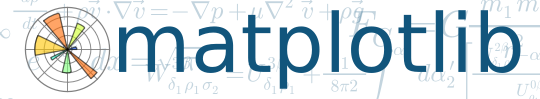
\includegraphics[height=0.1\textheight]{matplotlib-logo.png}
\;

\includegraphics[height=0.1\textheight]{python-logo.png}
\end{center}
\end{frame}

\begin{frame}
\frametitle{Example : an Enzymatic Reaction : Overview of System}
\begin{block}{Enzymatic Reaction}
The enzyme $E$ acts as a catalyst for the transformation of the substrate $S$
into the product $P$, via the complex $C$:
\begin{equation*}
S + E \leftrightarrow{} C \rightarrow{} P + E \; .
\end{equation*}

System consists of three reactions:
\begin{gather*}
S + E \xrightarrow[]{k_1} C \; , \qquad{}
C \xrightarrow[]{k_2} S + E \; , \qquad{}
C \xrightarrow[]{k_3} P + E \; .
\end{gather*} 

Kinetic parameters: $k_1 = 0.01, k_2 = 35, k_3 = 30$.

Initial species copy counts: $S_0 = 50, E_0 = 10, C_0 = 0, P_0 = 0$.
\end{block}
\end{frame}

\begin{frame}
\frametitle{Example : an Enzymatic Reaction : Modelling the System}
\framesubtitle{Species Count Functions}
\begin{block}{Defining the State Space}
Let $[S] \in \mathbb{N}$ denote the species count of the species
$S$ (similarly for $C, E, P$).

Define the states in the state space by
$(x_0, x_1) := ([S], [C]) \in \mathbb{N}^2$.
\end{block}
\begin{block}{Species Count Functions}
All species counts can be expressed in terms of the state $(x_0, x_1)$:
\begin{align*}
[S](x_0, x_1) & := x_0 \; , \\
[E](x_0, x_1) & := E_0 - x_1 \; , \\
[C](x_0, x_1) & := x_1 \; , \\
[P](x_0, x_1) & := S_0 - x_0 - x_1 \; .
\end{align*}
\end{block}
\end{frame}

\begin{frame}[fragile]
\frametitle{Example : an Enzymatic Reaction : Modelling the System}
\framesubtitle{Species Count Functions}
\begin{block}{Species Count Functions in Python}
\begin{Verbatim}[commandchars=\\\{\}]
\PYG{n}{s\PYGZus{}0} \PYG{o}{=} \PYG{l+m+mi}{50}
\PYG{n}{e\PYGZus{}0} \PYG{o}{=} \PYG{l+m+mi}{10}

\PYG{n}{s} \PYG{o}{=} \PYG{k}{lambda} \PYG{o}{*}\PYG{n}{x} \PYG{p}{:} \PYG{n}{x}\PYG{p}{[}\PYG{l+m+mi}{0}\PYG{p}{]}
\PYG{n}{e} \PYG{o}{=} \PYG{k}{lambda} \PYG{o}{*}\PYG{n}{x} \PYG{p}{:} \PYG{n}{e\PYGZus{}0} \PYG{o}{-} \PYG{n}{x}\PYG{p}{[}\PYG{l+m+mi}{1}\PYG{p}{]}
\PYG{n}{c} \PYG{o}{=} \PYG{k}{lambda} \PYG{o}{*}\PYG{n}{x} \PYG{p}{:} \PYG{n}{x}\PYG{p}{[}\PYG{l+m+mi}{1}\PYG{p}{]}
\PYG{n}{p} \PYG{o}{=} \PYG{k}{lambda} \PYG{o}{*}\PYG{n}{x} \PYG{p}{:} \PYG{n}{s\PYGZus{}0} \PYG{o}{-} \PYG{n}{x}\PYG{p}{[}\PYG{l+m+mi}{0}\PYG{p}{]} \PYG{o}{-} \PYG{n}{x}\PYG{p}{[}\PYG{l+m+mi}{1}\PYG{p}{]}
\end{Verbatim}
\end{block}
\end{frame}

\begin{frame}[fragile]
\frametitle{Example : an Enzymatic Reaction : Modelling the System}
\framesubtitle{Reaction Propensity Functions}
\begin{block}{Reaction Propensity Functions}
We can express the propensity functions $\nu_1, \nu_2, \nu_3$ of the
three reactions as functions of the state $(x_0, x_1) \in \mathbb{N}^2$ :
\begin{align*}
\nu_1(x_0, x_1) := & 0.01 \cdot [S](x_0, x_1) \cdot [E](x_0, x_1) \; , \\
\nu_2(x_0, x_1) := & 35 \cdot [C](x_0, x_1) \; ,\\
\nu_3(x_0, x_1) := & 30 \cdot [C](x_0, x_1) \; .
\end{align*}
\end{block}
\begin{block}{Reaction Propensity Functions in Python}
\begin{Verbatim}[commandchars=\\\{\}]
\PYG{n}{propensities} \PYG{o}{=} \PYG{p}{(}
    \PYG{k}{lambda} \PYG{o}{*}\PYG{n}{x} \PYG{p}{:} \PYG{l+m+mf}{0.01}\PYG{o}{*}\PYG{n}{s}\PYG{p}{(}\PYG{o}{*}\PYG{n}{x}\PYG{p}{)}\PYG{o}{*}\PYG{n}{e}\PYG{p}{(}\PYG{o}{*}\PYG{n}{x}\PYG{p}{)}\PYG{p}{,}
    \PYG{k}{lambda} \PYG{o}{*}\PYG{n}{x} \PYG{p}{:} \PYG{l+m+mf}{35.0}\PYG{o}{*}\PYG{n}{c}\PYG{p}{(}\PYG{o}{*}\PYG{n}{x}\PYG{p}{)}\PYG{p}{,}
    \PYG{k}{lambda} \PYG{o}{*}\PYG{n}{x} \PYG{p}{:} \PYG{l+m+mf}{30.0}\PYG{o}{*}\PYG{n}{c}\PYG{p}{(}\PYG{o}{*}\PYG{n}{x}\PYG{p}{)}\PYG{p}{,}
\PYG{p}{)}
\end{Verbatim}
\end{block}
\end{frame}

\begin{frame}[fragile]
\frametitle{Example : an Enzymatic Reaction : Modelling the System}
\framesubtitle{Reaction State Transitions}
\begin{block}{Reaction State Transitions}
The first reaction $S + E \xrightarrow[]{} C$ reduces the copy counts of
$S$ and $E$ by one, but increases the copy count of $C$ by one.
In terms of $(x_0, x_1) = ([S], [C])$ coordinates, the corresponding transition
is:
\begin{equation*}
(x_0, x_1) \mapsto (x_0 - 1, x_1 + 1) = (x_0, x_1) + (-1, 1)
\end{equation*}
The transitions for the second and third reactions are
$(1, -1), (0, -1)$.
\end{block}
\begin{block}{Reaction State Transitions in Python}
\begin{Verbatim}[commandchars=\\\{\}]
\PYG{n}{transitions} \PYG{o}{=} \PYG{p}{(}
    \PYG{p}{(}\PYG{o}{-}\PYG{l+m+mi}{1}\PYG{p}{,} \PYG{l+m+mi}{1}\PYG{p}{)}\PYG{p}{,}
    \PYG{p}{(}\PYG{l+m+mi}{1}\PYG{p}{,} \PYG{o}{-}\PYG{l+m+mi}{1}\PYG{p}{)}\PYG{p}{,}
    \PYG{p}{(}\PYG{l+m+mi}{0}\PYG{p}{,} \PYG{o}{-}\PYG{l+m+mi}{1}\PYG{p}{)}
\PYG{p}{)}
\end{Verbatim}
\end{block}
\end{frame}

\begin{frame}[fragile]
\frametitle{Example : an Enzymatic Reaction : Modelling the System}
\framesubtitle{The Complete Model}
\begin{columns}[t]
\column{0.45\textwidth}
\begin{block}{First, Define Species Counts}
\begin{Verbatim}[commandchars=\\\{\}, fontsize=\tiny]
\PYG{n}{s\PYGZus{}0} \PYG{o}{=} \PYG{l+m+mi}{50}
\PYG{n}{e\PYGZus{}0} \PYG{o}{=} \PYG{l+m+mi}{10}

\PYG{n}{s} \PYG{o}{=} \PYG{k}{lambda} \PYG{o}{*}\PYG{n}{x} \PYG{p}{:} \PYG{n}{x}\PYG{p}{[}\PYG{l+m+mi}{0}\PYG{p}{]}
\PYG{n}{e} \PYG{o}{=} \PYG{k}{lambda} \PYG{o}{*}\PYG{n}{x} \PYG{p}{:} \PYG{n}{e\PYGZus{}0} \PYG{o}{-} \PYG{n}{x}\PYG{p}{[}\PYG{l+m+mi}{1}\PYG{p}{]}
\PYG{n}{c} \PYG{o}{=} \PYG{k}{lambda} \PYG{o}{*}\PYG{n}{x} \PYG{p}{:} \PYG{n}{x}\PYG{p}{[}\PYG{l+m+mi}{1}\PYG{p}{]}
\PYG{n}{p} \PYG{o}{=} \PYG{k}{lambda} \PYG{o}{*}\PYG{n}{x} \PYG{p}{:} \PYG{n}{s\PYGZus{}0} \PYG{o}{-} \PYG{n}{x}\PYG{p}{[}\PYG{l+m+mi}{0}\PYG{p}{]} \PYG{o}{-} \PYG{n}{x}\PYG{p}{[}\PYG{l+m+mi}{1}\PYG{p}{]}
\end{Verbatim}
\end{block}
\begin{block}{Model Attributes}
The \verb+shape+ attribute defines (exclusive) upper bounds on the
$(x_0, x_1)$ coordinates, while the \verb+initial_state+ attribute specifies
initial conditions for the CME.
\end{block}
\column{0.55\textwidth}
\begin{block}{Second, Define Model}
\begin{Verbatim}[commandchars=\\\{\}, fontsize=\tiny]
\PYG{k+kn}{from} \PYG{n+nn}{cmepy} \PYG{k+kn}{import} \PYG{n}{model}

\PYG{n}{m} \PYG{o}{=} \PYG{n}{model}\PYG{o}{.}\PYG{n}{create}\PYG{p}{(}
    \PYG{n}{species\PYGZus{}counts} \PYG{o}{=} \PYG{p}{(}\PYG{n}{s}\PYG{p}{,} \PYG{n}{e}\PYG{p}{,} \PYG{n}{c}\PYG{p}{,} \PYG{n}{p}\PYG{p}{,} \PYG{p}{)}\PYG{p}{,}
    \PYG{n}{propensities} \PYG{o}{=} \PYG{p}{(}
        \PYG{k}{lambda} \PYG{o}{*}\PYG{n}{x} \PYG{p}{:} \PYG{l+m+mf}{0.01}\PYG{o}{*}\PYG{n}{s}\PYG{p}{(}\PYG{o}{*}\PYG{n}{x}\PYG{p}{)}\PYG{o}{*}\PYG{n}{e}\PYG{p}{(}\PYG{o}{*}\PYG{n}{x}\PYG{p}{)}\PYG{p}{,}
        \PYG{k}{lambda} \PYG{o}{*}\PYG{n}{x} \PYG{p}{:} \PYG{l+m+mf}{35.0}\PYG{o}{*}\PYG{n}{c}\PYG{p}{(}\PYG{o}{*}\PYG{n}{x}\PYG{p}{)}\PYG{p}{,}
        \PYG{k}{lambda} \PYG{o}{*}\PYG{n}{x} \PYG{p}{:} \PYG{l+m+mf}{30.0}\PYG{o}{*}\PYG{n}{c}\PYG{p}{(}\PYG{o}{*}\PYG{n}{x}\PYG{p}{)}\PYG{p}{,}
    \PYG{p}{)}\PYG{p}{,}
    \PYG{n}{transitions} \PYG{o}{=} \PYG{p}{(}
        \PYG{p}{(}\PYG{o}{-}\PYG{l+m+mi}{1}\PYG{p}{,} \PYG{l+m+mi}{1}\PYG{p}{)}\PYG{p}{,}
        \PYG{p}{(}\PYG{l+m+mi}{1}\PYG{p}{,} \PYG{o}{-}\PYG{l+m+mi}{1}\PYG{p}{)}\PYG{p}{,}
        \PYG{p}{(}\PYG{l+m+mi}{0}\PYG{p}{,} \PYG{o}{-}\PYG{l+m+mi}{1}\PYG{p}{)}
    \PYG{p}{)}\PYG{p}{,}
    \PYG{n}{shape} \PYG{o}{=} \PYG{p}{(}\PYG{n}{s\PYGZus{}0} \PYG{o}{+} \PYG{l+m+mi}{1}\PYG{p}{,} \PYG{n+nb}{min}\PYG{p}{(}\PYG{n}{s\PYGZus{}0}\PYG{p}{,} \PYG{n}{e\PYGZus{}0}\PYG{p}{)} \PYG{o}{+} \PYG{l+m+mi}{1}\PYG{p}{)}\PYG{p}{,}
    \PYG{n}{initial\PYGZus{}state} \PYG{o}{=} \PYG{p}{(}\PYG{n}{s\PYGZus{}0}\PYG{p}{,} \PYG{l+m+mi}{0}\PYG{p}{)}
\PYG{p}{)}
\end{Verbatim}
\end{block}
\end{columns}
\end{frame}


\begin{frame}[fragile]
\frametitle{Example : an Enzymatic Reaction : Solving the Model}
\begin{block}{Solving the Enzymatic Reaction Model}
\begin{Verbatim}[commandchars=\\\{\}]
\PYG{k+kn}{import} \PYG{n+nn}{numpy}
\PYG{k+kn}{from} \PYG{n+nn}{cmepy} \PYG{k+kn}{import} \PYG{n}{solver}

\PYG{n}{enzyme\PYGZus{}solver} \PYG{o}{=} \PYG{n}{solver}\PYG{o}{.}\PYG{n}{create}\PYG{p}{(}
    \PYG{n}{model} \PYG{o}{=} \PYG{n}{m}\PYG{p}{,}
    \PYG{n}{sink} \PYG{o}{=} \PYG{n+nb+bp}{False}
\PYG{p}{)}

\PYG{n}{time\PYGZus{}steps} \PYG{o}{=} \PYG{n}{numpy}\PYG{o}{.}\PYG{n}{linspace}\PYG{p}{(}\PYG{l+m+mf}{0.0}\PYG{p}{,} \PYG{l+m+mf}{10.0}\PYG{p}{,} \PYG{l+m+mi}{101}\PYG{p}{)}

\PYG{k}{for} \PYG{n}{t} \PYG{o+ow}{in} \PYG{n}{time\PYGZus{}steps}\PYG{p}{:}
    \PYG{n}{enzyme\PYGZus{}solver}\PYG{o}{.}\PYG{n}{step}\PYG{p}{(}\PYG{n}{t}\PYG{p}{)}
\end{Verbatim}
\end{block}
\end{frame}

\begin{frame}[fragile]
\frametitle{Example : an Enzymatic Reaction : Results}
\begin{block}{Computing and Displaying Results}
\begin{Verbatim}[commandchars=\\\{\}]
\PYG{k+kn}{from} \PYG{n+nn}{cmepy} \PYG{k+kn}{import} \PYG{n}{recorder}
\PYG{n}{r} \PYG{o}{=} \PYG{n}{recorder}\PYG{o}{.}\PYG{n}{create}\PYG{p}{(}
    \PYG{p}{(}\PYG{p}{[}\PYG{l+s}{'}\PYG{l+s}{S}\PYG{l+s}{'}\PYG{p}{,} \PYG{l+s}{'}\PYG{l+s}{E}\PYG{l+s}{'}\PYG{p}{,} \PYG{l+s}{'}\PYG{l+s}{C}\PYG{l+s}{'}\PYG{p}{,} \PYG{l+s}{'}\PYG{l+s}{P}\PYG{l+s}{'}\PYG{p}{]}\PYG{p}{,} \PYG{n}{m}\PYG{o}{.}\PYG{n}{species\PYGZus{}counts}\PYG{p}{)}
\PYG{p}{)}

\PYG{k}{for} \PYG{n}{t} \PYG{o+ow}{in} \PYG{n}{time\PYGZus{}steps}\PYG{p}{:}
    \PYG{n}{enzyme\PYGZus{}solver}\PYG{o}{.}\PYG{n}{step}\PYG{p}{(}\PYG{n}{t}\PYG{p}{)}
    \PYG{n}{r}\PYG{o}{.}\PYG{n}{write}\PYG{p}{(}\PYG{n}{t}\PYG{p}{,} \PYG{n}{enzyme\PYGZus{}solver}\PYG{o}{.}\PYG{n}{y}\PYG{p}{)}

\PYG{n}{recorder}\PYG{o}{.}\PYG{n}{display\PYGZus{}plots}\PYG{p}{(}\PYG{n}{r}\PYG{p}{)}
\end{Verbatim}
\end{block}
\end{frame}

\begin{frame}
\frametitle{Example : an Enzymatic Reaction : Results}
\begin{block}{Expected Values of Species Counts}
\begin{center}
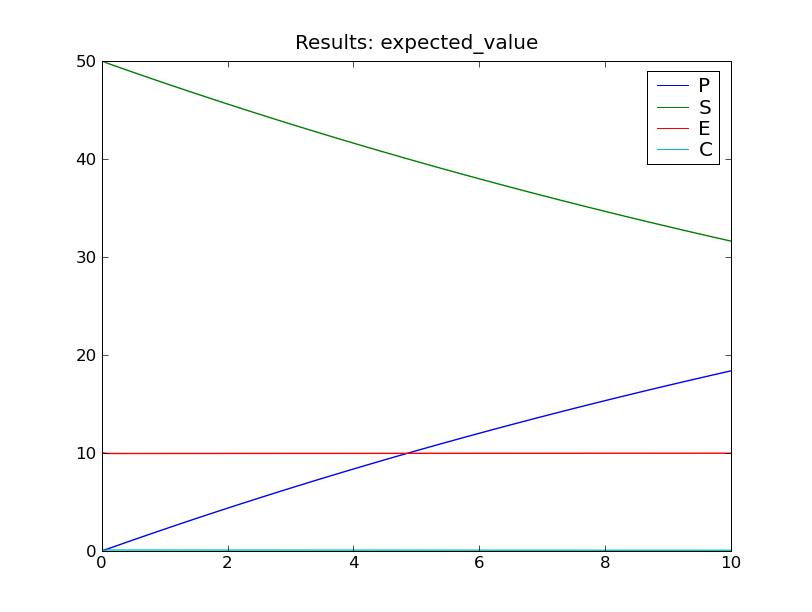
\includegraphics[height=0.75\textheight]{results_ev.png}
\end{center}
\end{block}

\end{frame}

\begin{frame}
\frametitle{Example : an Enzymatic Reaction : Results}
\begin{block}{Expected Values of Species Counts}
\begin{center}
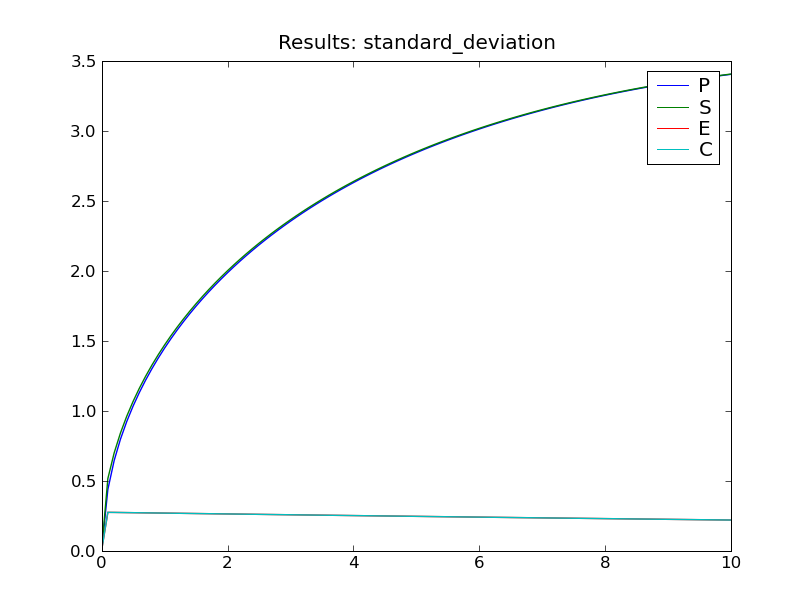
\includegraphics[height=0.75\textheight]{results_std_dev.png}
\end{center}
\end{block}
\end{frame}

\begin{frame}
\frametitle{Summary of CmePy Features}
\begin{block}{CmePy Features}
\begin{itemize}
\item models can be defined using species or reaction counts
\item both dense `rectangular' and sparse state spaces are supported
\item error due to state space truncation may be tracked with an FSP-style
`sink' state
\item separable time-dependent reaction propensities are supported
\item common statistical results (expected values, standard deviation,
joint and marginal distributions, covariance) are easily obtained
\item documentation!
\end{itemize}
\end{block}
\end{frame}

\begin{frame}
\frametitle{CmePy Links}
\begin{block}{CmePy Links}
\begin{itemize}
\item Check out the code at CmePy's GitHub repository:
\begin{center}
\href{http://github.com/fcostin/cmepy/}{http://github.com/fcostin/cmepy/}
\end{center} 
\item Online documentation, including a number of extensive examples,
is available at:
\begin{center}
\href{http://fcostin.github.com/cmepy/}{http://fcostin.github.com/cmepy/}
\end{center}
\end{itemize}
\end{block}
\end{frame}
\end{document}
